\documentclass{standalone}
\usepackage{tikz}
\begin{document}
\begin{tikzpicture}
  \draw
    (2,0)
    -- (3,0)
    -- (4,0)
    -- (5,0)
    -- (6,0)
    -- (7,0)
    -- (8,0)
    -- (9,0)
    -- (10,0)
    -- (11,0)
    -- (12,0)
    -- (13,0)
    -- (14,0)
    -- (15,0)
    -- (16,0)
    -- (17,0)
    -- (18,0)
    -- (19,0)
    -- (20,0)
    -- (21,0)
    -- (22,0)
    -- (23,0)
    -- (24,0)
    -- (25,0)
    -- (26,0)
    -- (27,0)
    -- (28,0)
    -- (29,0)
    -- (30,0)
    -- (31,0)
    -- (32,0)
    -- (33,0)
    -- (34,0)
    -- (35,0)
    -- (36,0)
    -- (37,0)
    -- (38,0)
    -- (39,0)
    -- (40,0)
    -- (41,0)
    -- (42,0)
    -- (43,0)
    -- (44,0)
    -- (45,0)
    -- (46,0)
    -- (47,0)
    -- (48,0)
    -- (49,0) % Deleting this row makes the last row indent correctly
    ;
\end{tikzpicture}
\end{document}
